\documentclass[8pt,aspectratio=169]{beamer}
\usetheme{Madrid}
\usepackage{graphicx,booktabs,adjustbox,multicol,amsmath,amssymb,listings,xcolor}
\definecolor{mlblue}{RGB}{0,102,204}
\definecolor{mlpurple}{RGB}{51,51,178}
\definecolor{mllavender}{RGB}{173,173,224}
\definecolor{mllavender2}{RGB}{193,193,232}
\definecolor{mllavender3}{RGB}{204,204,235}
\definecolor{mllavender4}{RGB}{214,214,239}
\definecolor{mlorange}{RGB}{255,127,14}
\definecolor{mlgreen}{RGB}{44,160,44}
\definecolor{mlred}{RGB}{214,39,40}
\definecolor{mlgray}{RGB}{127,127,127}
\definecolor{solkeyword}{RGB}{0,102,153}
\setbeamercolor{palette primary}{bg=mllavender3,fg=mlpurple}
\setbeamercolor{palette secondary}{bg=mllavender2,fg=mlpurple}
\setbeamercolor{palette tertiary}{bg=mllavender,fg=white}
\setbeamercolor{palette quaternary}{bg=mlpurple,fg=white}
\setbeamercolor{structure}{fg=mlpurple}
\setbeamercolor{title}{fg=mlpurple}
\setbeamercolor{frametitle}{fg=mlpurple,bg=mllavender3}
\setbeamercolor{block title}{bg=mllavender2,fg=mlpurple}
\setbeamercolor{block body}{bg=mllavender4,fg=black}
\setbeamertemplate{navigation symbols}{}
\setbeamertemplate{itemize items}[circle]
\setbeamersize{text margin left=5mm,text margin right=5mm}
\newcommand{\bottomnote}[1]{\vfill\vspace{-2mm}\textcolor{mllavender2}{\rule{\textwidth}{0.4pt}}\vspace{1mm}\footnotesize\textbf{#1}}
\usepackage{tikz,pgfplots}
\pgfplotsset{compat=1.18}
\usetikzlibrary{arrows.meta,positioning,shapes.geometric,calc}
\title{ERC-20 Token Creation: Course Preview}
\subtitle{INTRO Preview}
\author{Prof.~Dr.~Joerg Osterrieder}
\institute{University Lecture Series}
\date{\today}
\begin{document}

% Frame 1: Title
\begin{frame}
\titlepage
\end{frame}

% Frame 2: Why Token Standards Matter
\begin{frame}{Why Token Standards Matter}
\begin{columns}[T]
\begin{column}{0.62\textwidth}
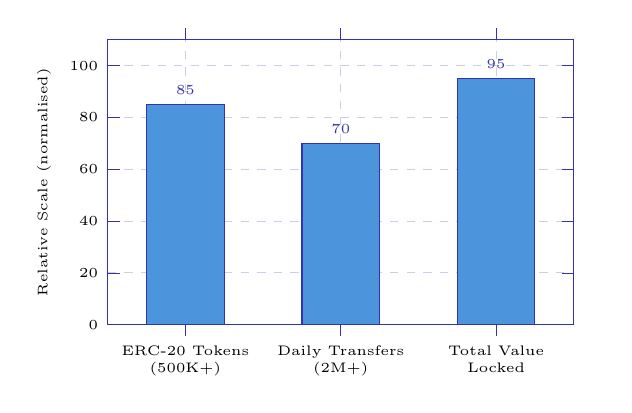
\begin{tikzpicture}
\begin{axis}[
  ybar,
  bar width=28pt,
  width=7.5cm,
  height=5.2cm,
  symbolic x coords={Tokens, Transfers, TVL},
  xtick=data,
  xticklabels={ERC-20 Tokens\\(500K+), Daily Transfers\\(2M+), Total Value\\Locked},
  xticklabel style={font=\tiny, text width=2.5cm, align=center},
  ymin=0, ymax=110,
  ytick={0,20,40,60,80,100},
  yticklabel style={font=\tiny},
  ylabel style={font=\tiny},
  ylabel={Relative Scale (normalised)},
  axis line style={draw=mlpurple},
  tick style={draw=mlpurple},
  nodes near coords,
  nodes near coords style={font=\tiny, color=mlpurple},
  point meta=y,
  enlarge x limits=0.25,
  grid=major,
  grid style={dashed, mllavender3},
]
\addplot[fill=mlblue!70, draw=mlpurple] coordinates {
  (Tokens,    85)
  (Transfers, 70)
  (TVL,       95)
};
\end{axis}
\end{tikzpicture}
\end{column}
\begin{column}{0.36\textwidth}
\vspace{4mm}
\begin{block}{Key Metrics}
\begin{itemize}\setlength\itemsep{4pt}
  \item[\small$\checkmark$] \small \textbf{500K+} ERC-20 tokens deployed
  \item[\small$\checkmark$] \small \textbf{2M+} token transfers per day
  \item[\small$\checkmark$] \small \textbf{90\%+} of DeFi TVL in ERC-20 assets
  \item[\small$\checkmark$] \small \textbf{Single standard} enables universal wallet support
\end{itemize}
\end{block}
\end{column}
\end{columns}
\bottomnote{ERC-20 is the most widely adopted token standard in crypto history}
\end{frame}

% Frame 3: The ERC-20 Interface at a Glance
\begin{frame}{The ERC-20 Interface at a Glance}
\vspace{2mm}
\begin{center}
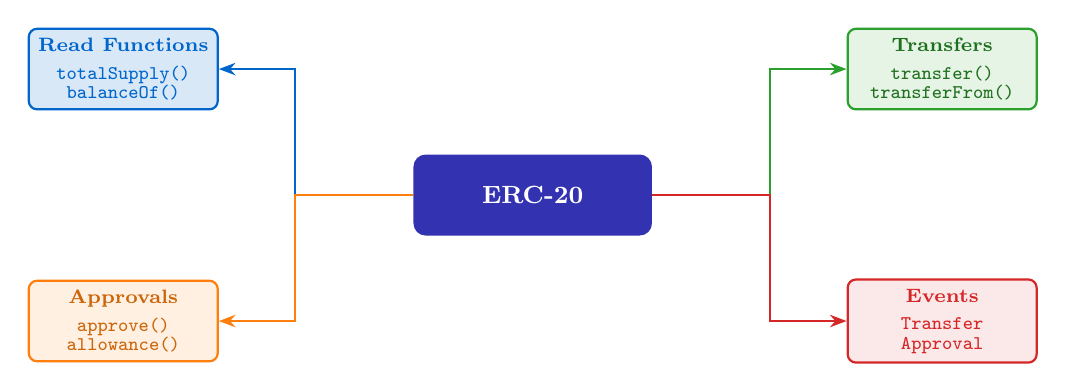
\begin{tikzpicture}[
  cbox/.style={rectangle, rounded corners=4pt, draw=mlpurple, thick,
               fill=mllavender3, minimum width=2.6cm, minimum height=0.8cm,
               font=\scriptsize\bfseries, align=center, text=mlpurple},
  rbox/.style={rectangle, rounded corners=3pt, thick,
               minimum width=2.4cm, minimum height=0.65cm,
               font=\scriptsize, align=center},
  arr/.style={-{Stealth[length=6pt]}, thick}
]
% Central box
\node[cbox, minimum width=3.0cm, minimum height=1.0cm,
      fill=mlpurple, text=white, font=\small\bfseries] (erc) at (0,0) {ERC-20};

% Read functions (top-left, mlblue)
\node[rbox, draw=mlblue, fill=mlblue!15, text=mlblue] (read) at (-5.2, 1.6)
  {\textbf{Read Functions}\\[2pt]\texttt{totalSupply()}\\[-1pt]\texttt{balanceOf()}};

% Transfer group (top-right, mlgreen)
\node[rbox, draw=mlgreen, fill=mlgreen!12, text=mlgreen!70!black] (trans) at (5.2, 1.6)
  {\textbf{Transfers}\\[2pt]\texttt{transfer()}\\[-1pt]\texttt{transferFrom()}};

% Approve group (bottom-left, mlorange)
\node[rbox, draw=mlorange, fill=mlorange!12, text=mlorange!80!black] (appr) at (-5.2,-1.6)
  {\textbf{Approvals}\\[2pt]\texttt{approve()}\\[-1pt]\texttt{allowance()}};

% Events group (bottom-right, mlred)
\node[rbox, draw=mlred, fill=mlred!10, text=mlred] (evts) at (5.2,-1.6)
  {\textbf{Events}\\[2pt]\texttt{Transfer}\\[-1pt]\texttt{Approval}};

% Arrows
\draw[arr, draw=mlblue]   (erc.west)  -- ++(-1.5,0) |- (read.east);
\draw[arr, draw=mlgreen]  (erc.east)  -- ++(1.5,0)  |- (trans.west);
\draw[arr, draw=mlorange] (erc.west)  -- ++(-1.5,0) |- (appr.east);
\draw[arr, draw=mlred]    (erc.east)  -- ++(1.5,0)  |- (evts.west);
\end{tikzpicture}
\end{center}
\bottomnote{Any contract implementing these 8 elements is ERC-20 compliant}
\end{frame}

% Frame 4: Token Economics Spectrum
\begin{frame}{Token Economics Spectrum}
\begin{columns}[T]
\begin{column}{0.62\textwidth}
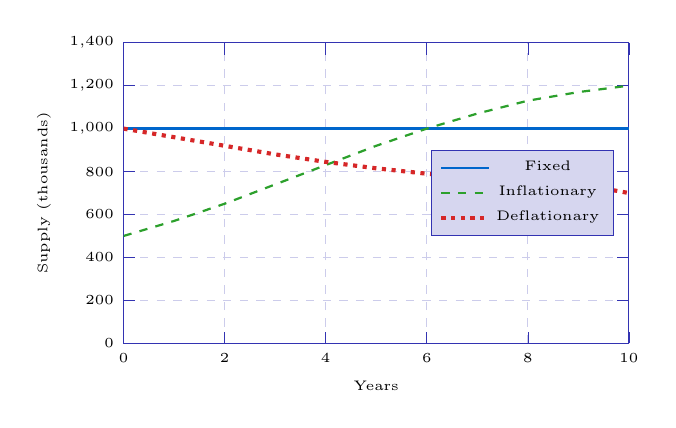
\begin{tikzpicture}
\begin{axis}[
  width=8.0cm,
  height=5.4cm,
  xmin=0, xmax=10,
  ymin=0, ymax=1400,
  xtick={0,2,4,6,8,10},
  ytick={0,200,400,600,800,1000,1200,1400},
  xticklabel style={font=\tiny},
  yticklabel style={font=\tiny},
  xlabel style={font=\tiny},
  ylabel style={font=\tiny},
  xlabel={Years},
  ylabel={Supply (thousands)},
  axis line style={draw=mlpurple},
  tick style={draw=mlpurple},
  grid=major,
  grid style={dashed, mllavender3},
  legend style={font=\tiny, at={(0.97,0.5)}, anchor=east,
                fill=mllavender4, draw=mlpurple},
]
% Fixed supply — flat at 1000
\addplot[color=mlblue, solid, thick] coordinates {
  (0,1000) (1,1000) (2,1000) (3,1000) (4,1000)
  (5,1000) (6,1000) (7,1000) (8,1000) (9,1000) (10,1000)
};
% Inflationary — grows from 500 to ~1200
\addplot[color=mlgreen, dashed, thick] coordinates {
  (0,500) (1,570) (2,650) (3,740) (4,830)
  (5,920) (6,1000) (7,1070) (8,1130) (9,1170) (10,1200)
};
% Deflationary — declines from 1000 to ~700
\addplot[color=mlred, dotted, thick, line width=1.5pt] coordinates {
  (0,1000) (1,960) (2,920) (3,880) (4,845)
  (5,815) (6,790) (7,770) (8,755) (9,742) (10,700)
};
\legend{Fixed, Inflationary, Deflationary}
\end{axis}
\end{tikzpicture}
\end{column}
\begin{column}{0.36\textwidth}
\vspace{4mm}
\begin{block}{Supply Models}
\begin{itemize}\setlength\itemsep{5pt}
  \item[\small$\checkmark$] \small \textcolor{mlblue}{\textbf{Fixed}} --- hard cap, predictable scarcity (e.g.\ BTC-like)
  \item[\small$\checkmark$] \small \textcolor{mlgreen!70!black}{\textbf{Inflationary}} --- minting rewards participants (e.g.\ staking tokens)
  \item[\small$\checkmark$] \small \textcolor{mlred}{\textbf{Deflationary}} --- burn mechanisms reduce supply over time
\end{itemize}
\end{block}
\end{column}
\end{columns}
\bottomnote{Supply model choice fundamentally shapes token value and adoption}
\end{frame}

% Frame 5: Course Coverage
\begin{frame}{Course Coverage}
\vspace{2mm}
\begin{center}
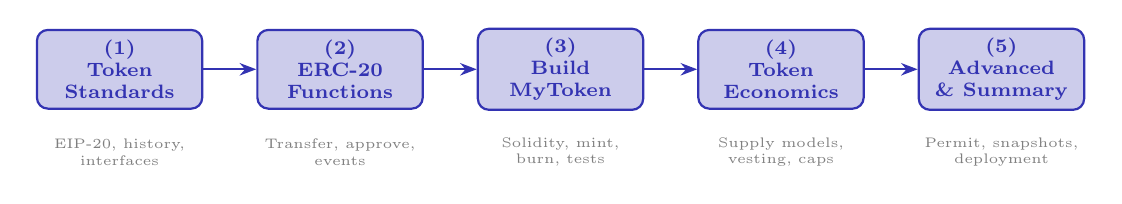
\begin{tikzpicture}[
  procstep/.style={
    rectangle, rounded corners=4pt,
    minimum width=2.1cm, minimum height=1.0cm,
    draw=mlpurple, thick,
    fill=mllavender3,
    font=\scriptsize\bfseries,
    align=center,
    text=mlpurple
  },
  conn/.style={-{Stealth[length=6pt]}, thick, draw=mlpurple}
]
\node[procstep] (s1) at (0,0)    {(1)\\Token\\Standards};
\node[procstep] (s2) at (2.8,0)  {(2)\\ERC-20\\Functions};
\node[procstep] (s3) at (5.6,0)  {(3)\\Build\\MyToken};
\node[procstep] (s4) at (8.4,0)  {(4)\\Token\\Economics};
\node[procstep] (s5) at (11.2,0) {(5)\\Advanced\\\& Summary};

\draw[conn] (s1) -- (s2);
\draw[conn] (s2) -- (s3);
\draw[conn] (s3) -- (s4);
\draw[conn] (s4) -- (s5);

\node[font=\tiny, text=mlgray, align=center, text width=2.1cm] at (0,-1.05)
  {EIP-20, history,\\interfaces};
\node[font=\tiny, text=mlgray, align=center, text width=2.1cm] at (2.8,-1.05)
  {Transfer, approve,\\events};
\node[font=\tiny, text=mlgray, align=center, text width=2.1cm] at (5.6,-1.05)
  {Solidity, mint,\\burn, tests};
\node[font=\tiny, text=mlgray, align=center, text width=2.1cm] at (8.4,-1.05)
  {Supply models,\\vesting, caps};
\node[font=\tiny, text=mlgray, align=center, text width=2.1cm] at (11.2,-1.05)
  {Permit, snapshots,\\deployment};
\end{tikzpicture}
\end{center}
\vspace{4mm}
\begin{columns}[T]
\begin{column}{0.48\textwidth}
\begin{block}{Prerequisites}
\begin{itemize}\setlength\itemsep{2pt}
  \item[\small$\checkmark$] \small Basic Solidity / programming knowledge
  \item[\small$\checkmark$] \small Familiarity with Ethereum accounts \& gas
\end{itemize}
\end{block}
\end{column}
\begin{column}{0.48\textwidth}
\begin{block}{Outcomes}
\begin{itemize}\setlength\itemsep{2pt}
  \item[\small$\checkmark$] \small Implement a fully compliant ERC-20 token
  \item[\small$\checkmark$] \small Design and deploy custom tokenomics
\end{itemize}
\end{block}
\end{column}
\end{columns}
\bottomnote{From standards to deployment in 55 frames}
\end{frame}

% Frame 6: What You Will Build
\begin{frame}{What You Will Build}
\begin{columns}[T]
\begin{column}{0.44\textwidth}
\vspace{2mm}
\begin{block}{Project Deliverables}
\begin{itemize}\setlength\itemsep{5pt}
  \item[\small$\checkmark$] \small \textbf{MyToken contract} --- full ERC-20 with mint \& burn
  \item[\small$\checkmark$] \small \textbf{Deploy script} --- Hardhat deployment to testnet
  \item[\small$\checkmark$] \small \textbf{Test suite} --- unit tests for all functions
  \item[\small$\checkmark$] \small \textbf{Tokenomics design} --- supply model \& vesting schedule
\end{itemize}
\end{block}
\end{column}
\begin{column}{0.54\textwidth}
\vspace{2mm}
\begin{center}
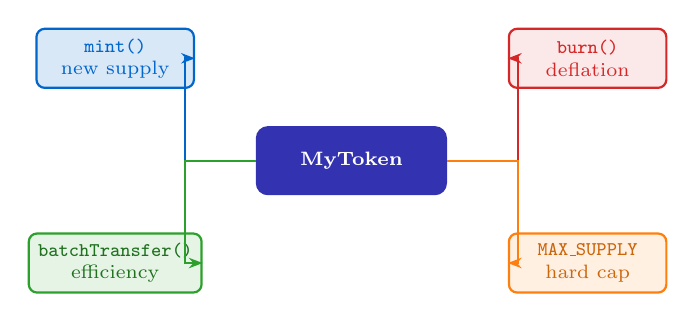
\begin{tikzpicture}[
  cbox/.style={rectangle, rounded corners=4pt, draw=mlpurple, thick,
               fill=mlpurple, minimum width=2.4cm, minimum height=0.85cm,
               font=\scriptsize\bfseries, align=center, text=white},
  fbox/.style={rectangle, rounded corners=3pt, thick,
               minimum width=2.0cm, minimum height=0.75cm,
               font=\scriptsize, align=center},
  farr/.style={-{Stealth[length=5pt]}, thick}
]
% Central node
\node[cbox] (mt) at (0,0) {MyToken};

% Feature nodes
\node[fbox, draw=mlblue, fill=mlblue!15, text=mlblue]      (mint) at (-3.0, 1.3) {\texttt{mint()}\\new supply};
\node[fbox, draw=mlred,  fill=mlred!10,  text=mlred]        (burn) at ( 3.0, 1.3) {\texttt{burn()}\\deflation};
\node[fbox, draw=mlgreen,fill=mlgreen!12,text=mlgreen!70!black] (batch) at (-3.0,-1.3) {\texttt{batchTransfer()}\\efficiency};
\node[fbox, draw=mlorange,fill=mlorange!12,text=mlorange!80!black] (cap)  at ( 3.0,-1.3) {\texttt{MAX\_SUPPLY}\\hard cap};

% Arrows
\draw[farr, draw=mlblue]   (mt.west)  -- ++(-0.9,0) |- (mint.east);
\draw[farr, draw=mlred]    (mt.east)  -- ++(0.9,0)  |- (burn.west);
\draw[farr, draw=mlgreen]  (mt.west)  -- ++(-0.9,0) |- (batch.east);
\draw[farr, draw=mlorange] (mt.east)  -- ++(0.9,0)  |- (cap.west);
\end{tikzpicture}
\end{center}
\end{column}
\end{columns}
\vspace{3mm}
\begin{center}
  \colorbox{mllavender3}{\parbox{0.82\textwidth}{\centering\small
    \textcolor{mlpurple}{\textbf{By the end:}} deploy your own ERC-20 token to a testnet
    and verify it on a block explorer.
  }}
\end{center}
\bottomnote{By the end you will deploy your own ERC-20 token to a testnet}
\end{frame}

\end{document}
